\section{Diagramme de classes}
Au cours de cette étude, plusieurs problématiques ont été soulevées; nous proposons donc un diagramme d'interfaces permettant de réponde au besoin exprimé lors de la présentation du sujet.
Ce diagramme présente toutes les fonctionnalités nécessaires pour le projet.
Nous y avons implémenté :
\begin{itemize}
  \item Un monteur pour la partie; le système permet de créer ou charger une partie et est extensible. 
		On pourrait rajouter une monteur pour créer un GameManager avec des conditions de victoire et de défaite supplémentaires.
  \item Une fabrique pour les différents peuples. Il est ainsi aisé de rajouter un peuple supplémentaire.
  \item Un poids-mouche pour l'utilisation du plateau de jeu. L'objectif est de réduire l'empreinte mémoire de notre jeu
  \item Un patron de conception strategie est utilisé pour la génération avec différentes tailles de carte.
  \item La sauvegarde implémente elle aussi stratégie : Il serait ainsi possible d'avoir différents formats de sauvegarde.
\end{itemize} 
Toutes ces informations sont détaillées sur diagramme d'interfaces \ref{fig:interfaceDiagram}.
\newline
\newline
\begin{figure}[h!]
    \centering
    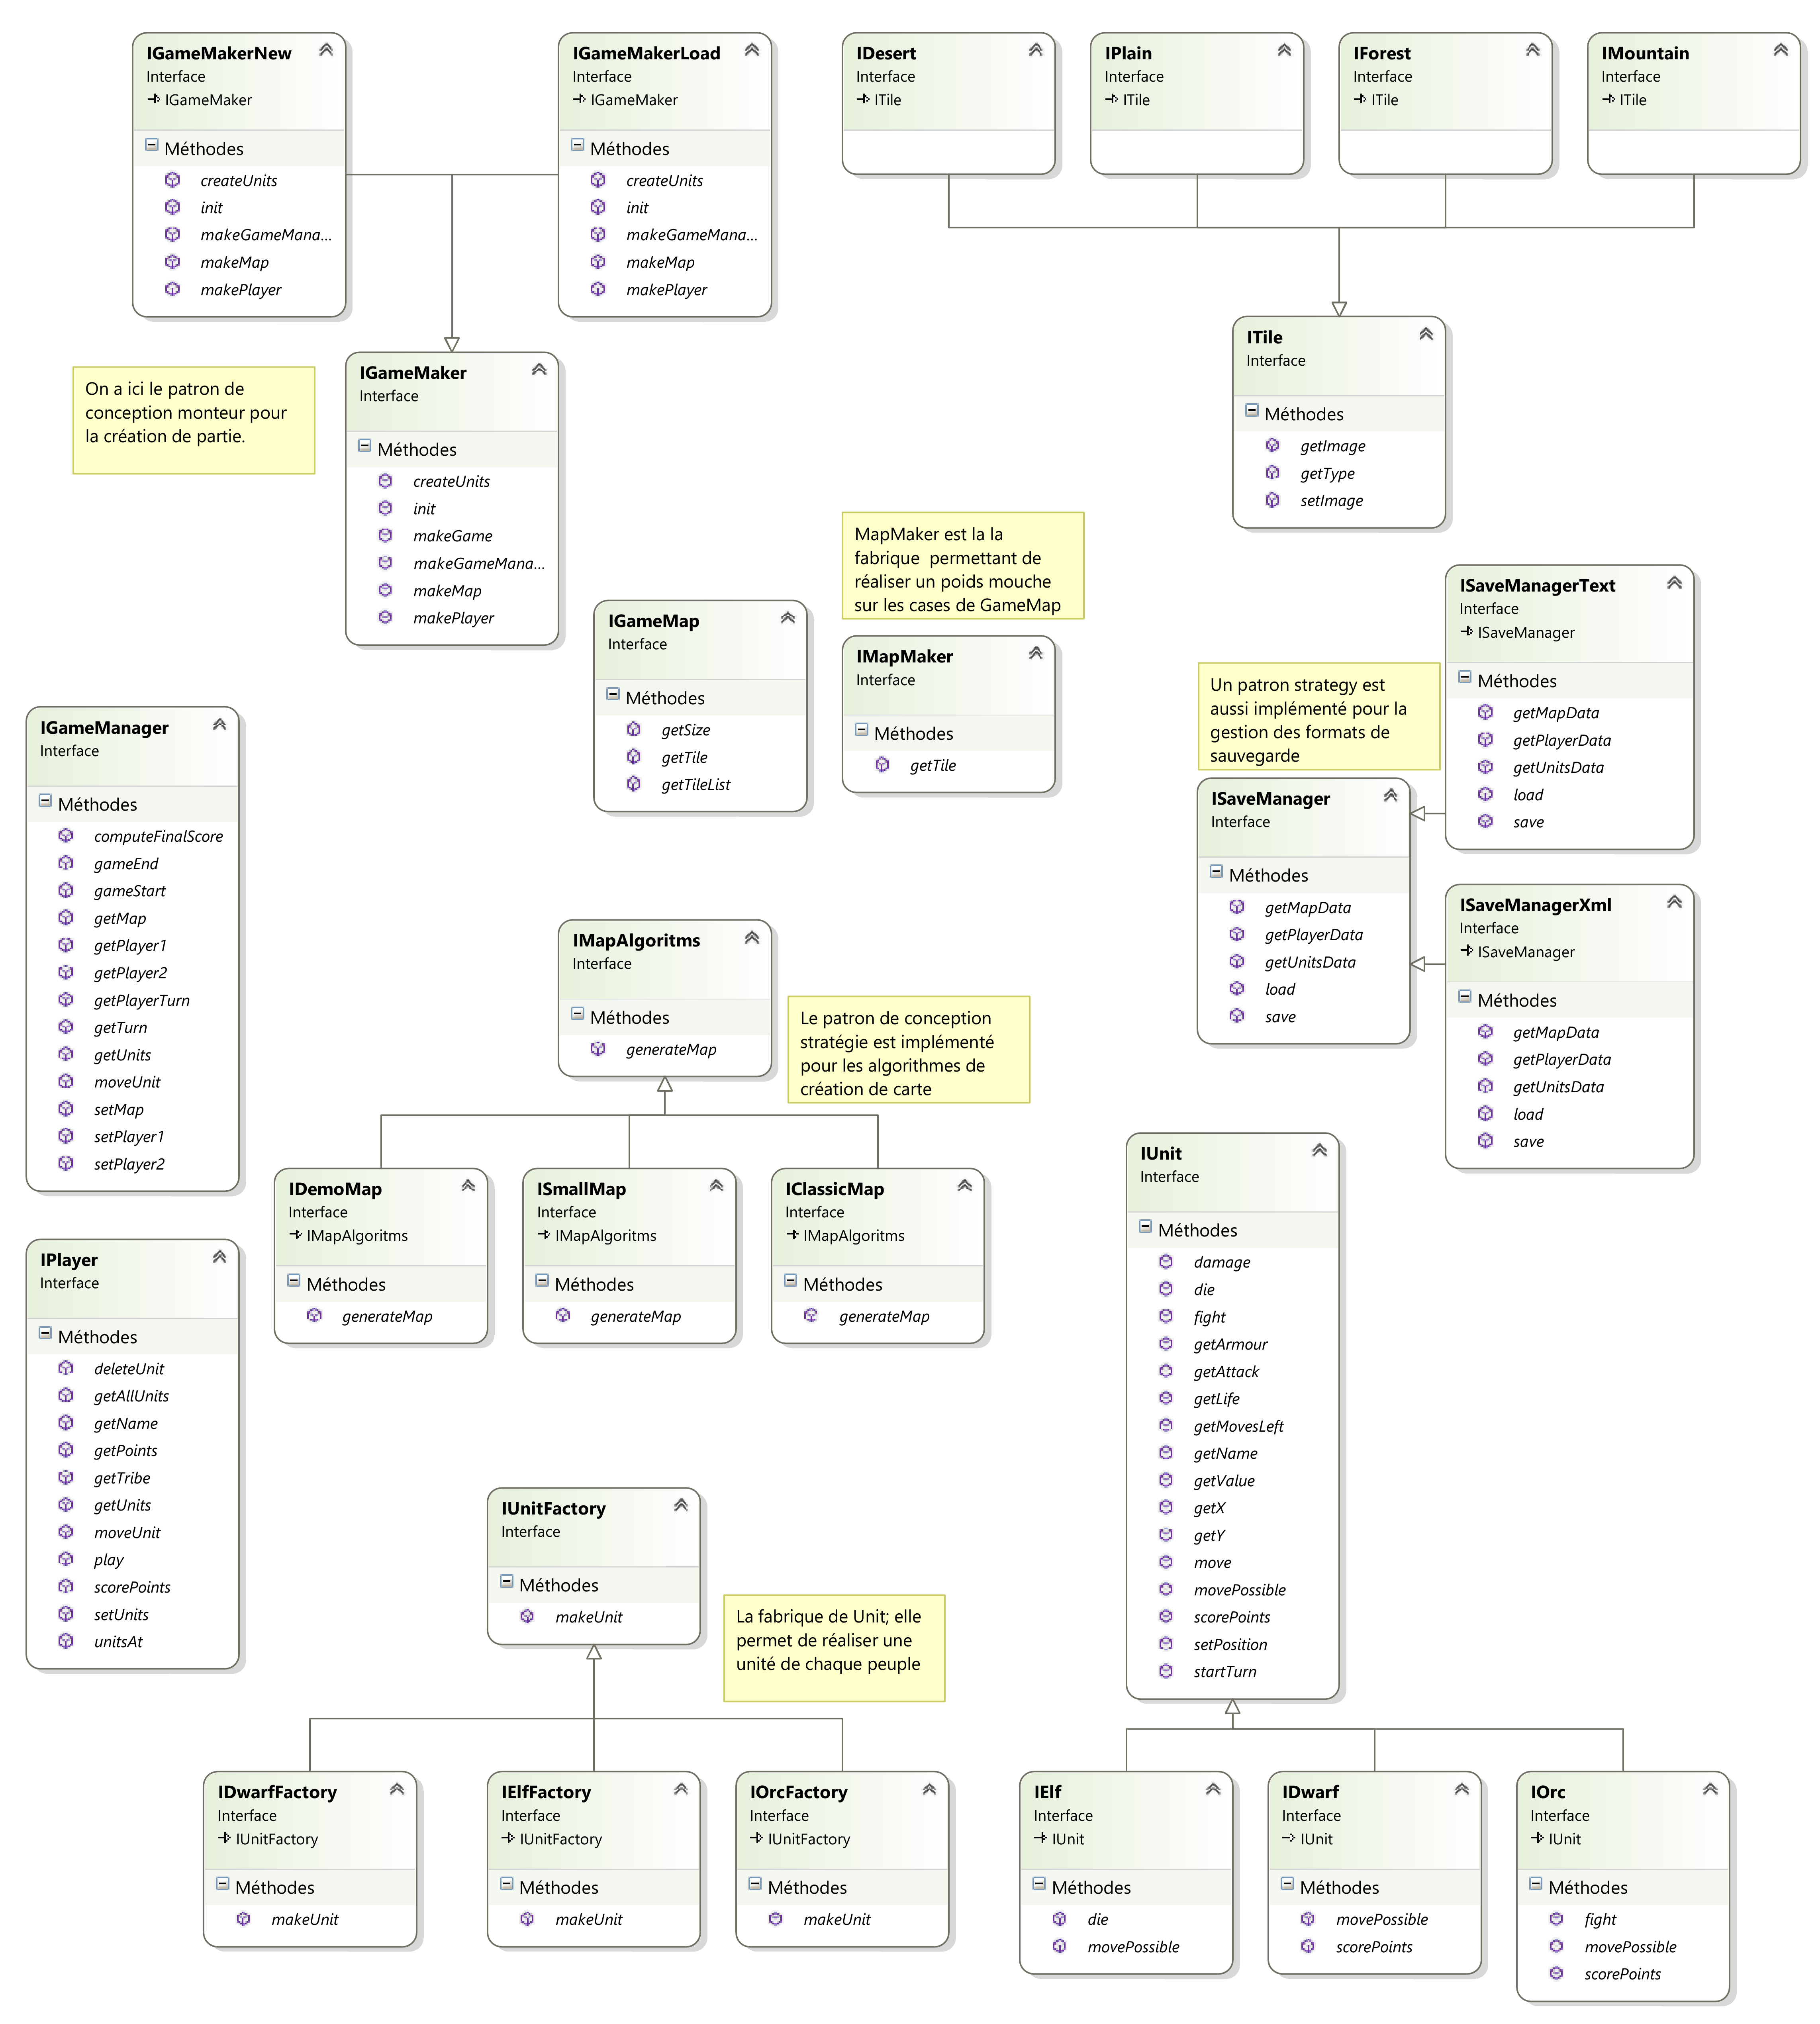
\includegraphics[width=0.8\textwidth]{res/Interfaces.png}
    \caption{Interfaces de programmation}
    \label{fig:interfaceDiagram}
\end{figure}

Les attributs nécessaires ont alors été rajoutés pour créer les classes.
Parmis les choix notables de réalisation, on citera : 
\begin{itemize}
  \item Utilisation d'une Dictionary<string, Tile> pour le poids-mouche. Le système est plus lourd que des membres statiques dans notre cas, mais il est plus extensible.
  \item Utilisation de la structure UnitData, pour une restauration plus facile des unités lors d'un chargement.
  \item Stocker les types de tiles dans une liste et non dans un tableau à deux dimensions; il est ainsi plus facile de controler le déplacement.
\end{itemize}
Tout ces détails sont visibles sur le diagramme de classe \ref{fig:classDiagram}.
\begin{figure}[h!]
    \centering
    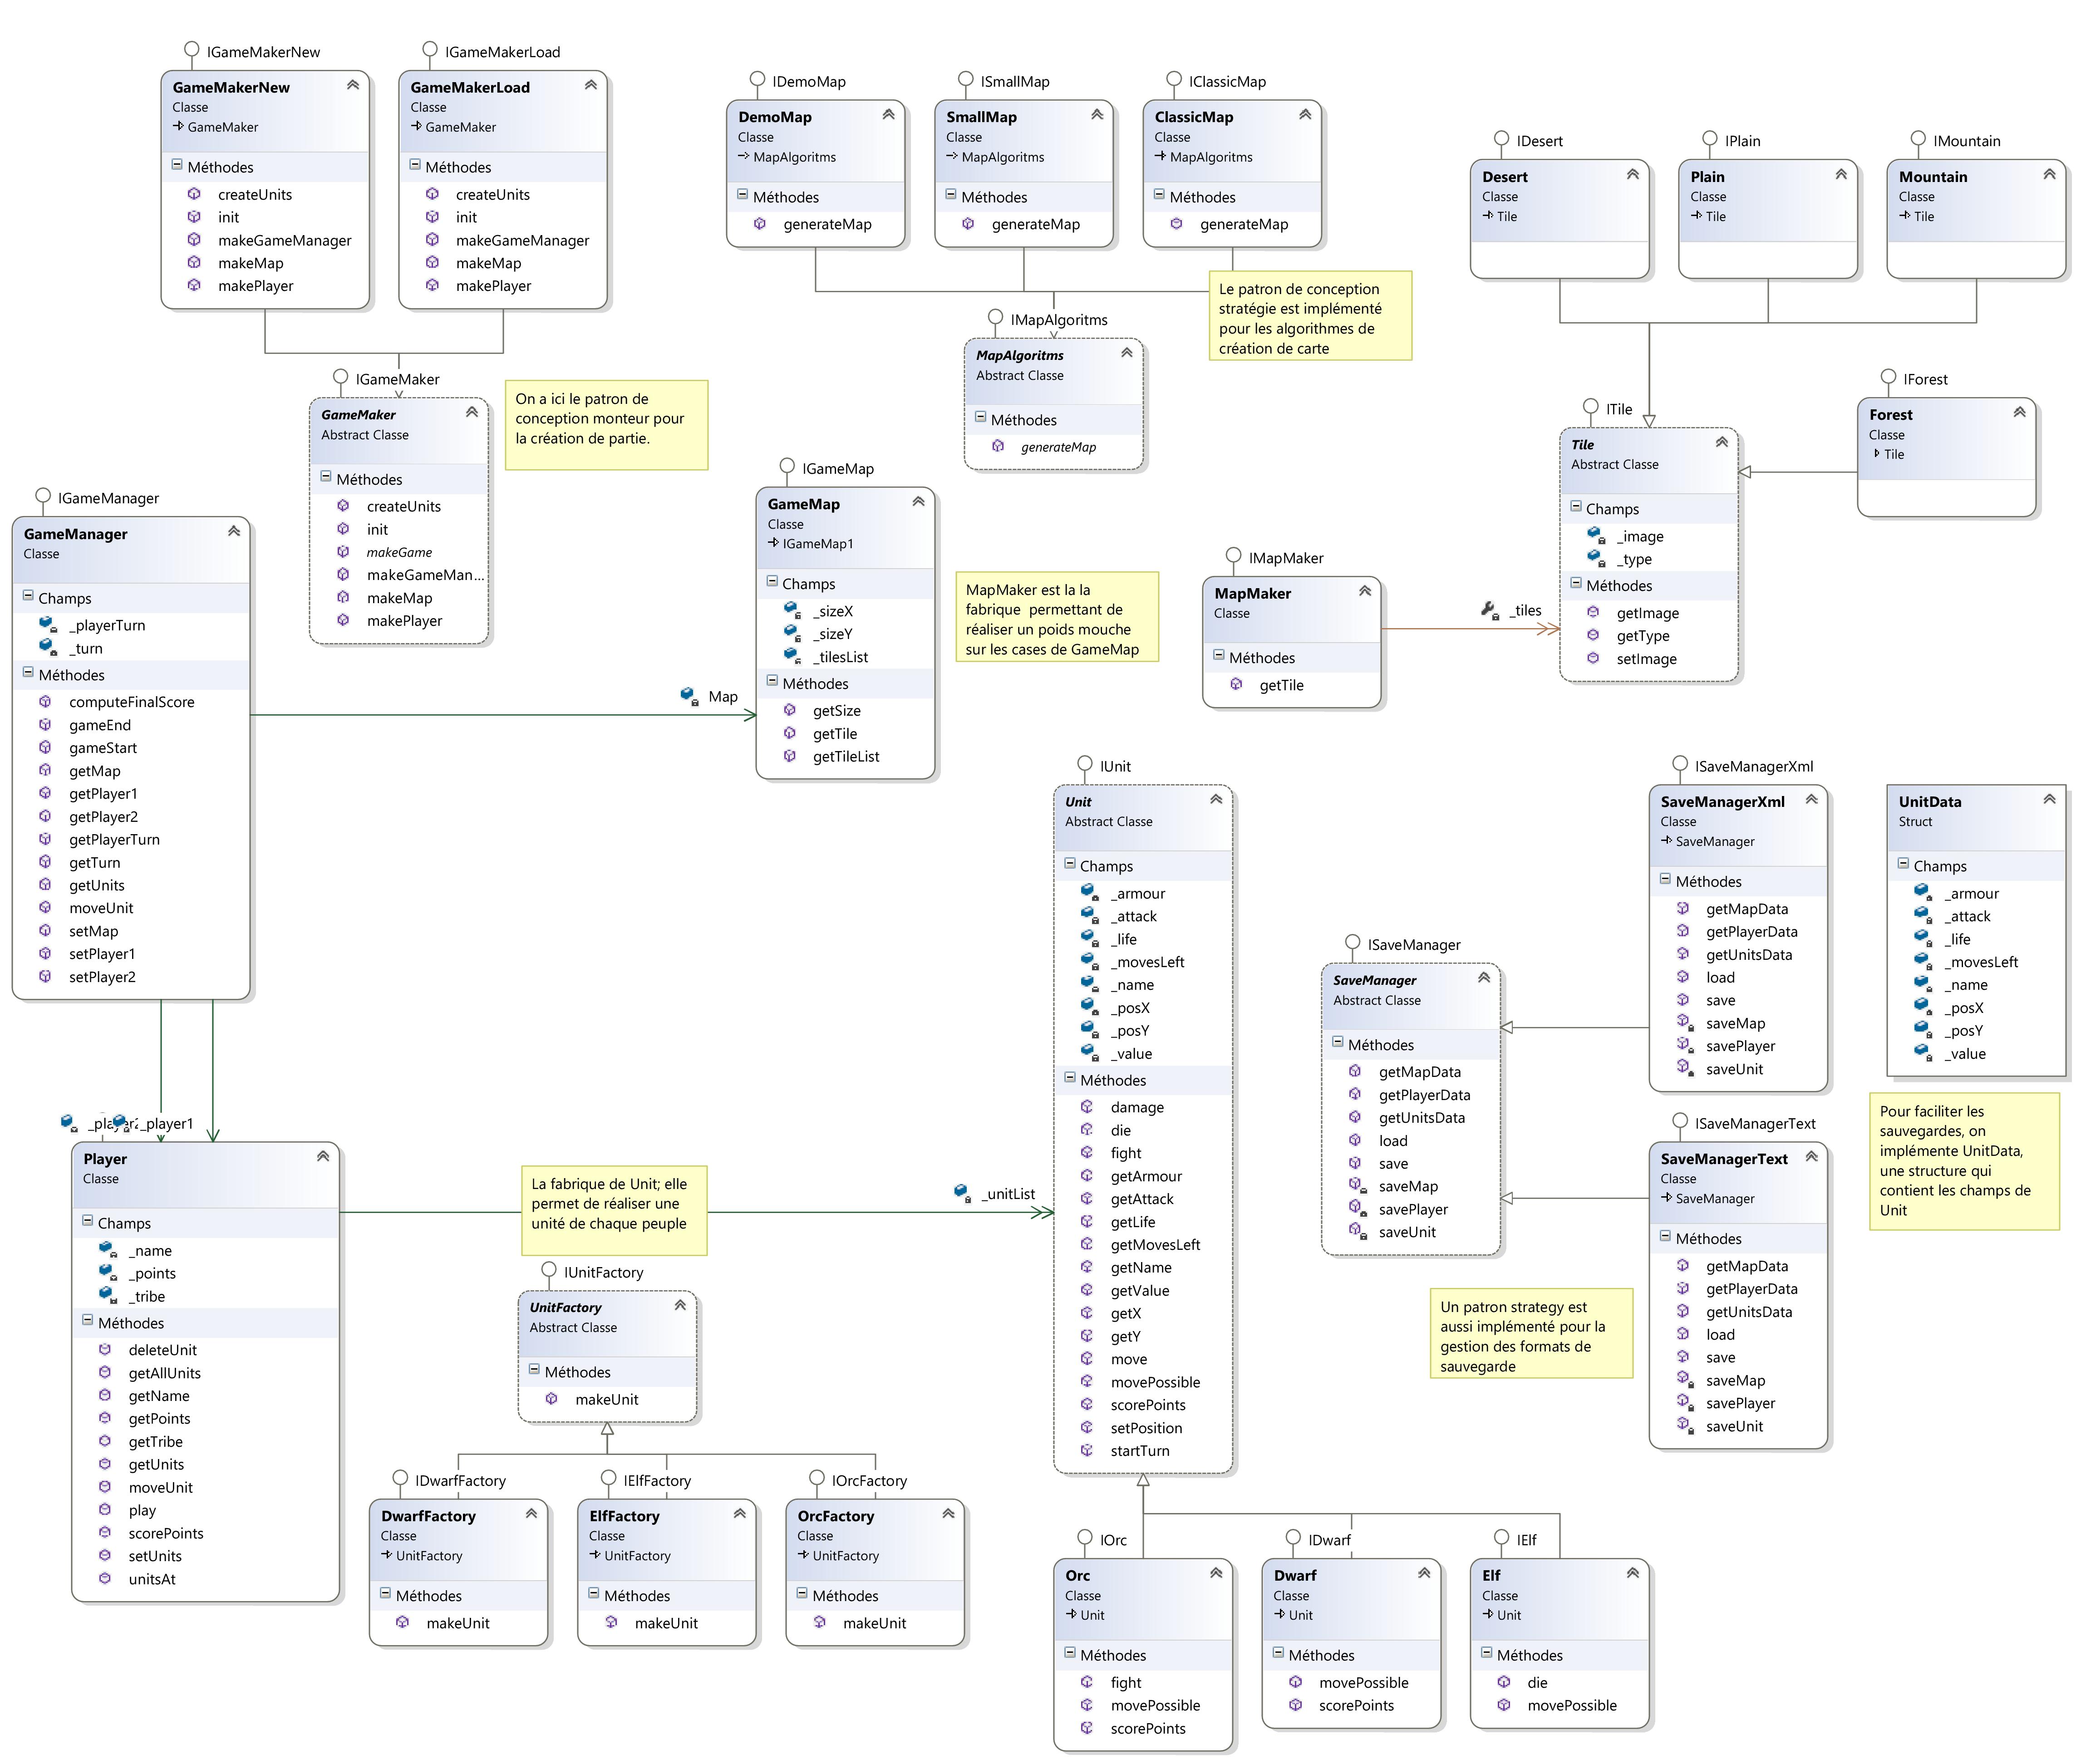
\includegraphics[width=0.8\textwidth]{res/Implementation.png}
    \caption{Diagramme de classes}
    \label{fig:classDiagram}
\end{figure}